 
\documentclass[titlepage, 12pt]{article}

\usepackage{framed}
\usepackage{enumitem}
\usepackage{geometry}
\geometry{
  letterpaper,
  margin=1in,
}

\usepackage{graphicx}
\graphicspath{{./images/}}
\usepackage{hyperref}
\usepackage{float}
% \usepackage{subcaption}
\usepackage{amssymb}

\title{SE 2XB3 Group 4 Report 6}
\author{
  Huang, Kehao \\
  400235182 \\
  \texttt{huangk53@mcmaster.ca} \\
  L01
  \and
  Jiao, Anhao \\
  400251837 \\
  \texttt{jiaoa3@mcmaster.ca} \\
  L01
  \and
  Ye, Xunzhou \\
  400268576 \\
  \texttt{yex33@mcmaster.ca} \\
  L01
}
\date{5 March 2021}

\begin{document}
\maketitle{}

\newpage{}

\section{Red-Black Tree Height}
\label{sec:rbh}

Due to the different implementations of red-black trees, our implementation of a
Left-Leaning Red-Black (LLRB) tree yield the heights 14, 26, and 16 for three
rounds of inserting the numbers 1 through 10,000. Nonetheless, an surprising
reduction in height along with an increase in element count is observed. There
are several factors causing this behaviour. First, the first stage of insertion
into a LLRB tree is the same as a Binary Search Tree (BST) insertion. In this
case where the numbers are inserted in an ascending order, it is the worst
scenario for both LLRB tree and BST. Therefore, after the \texttt{fix} stage in
an LLRB tree insertion, the LLRB tree would be at the worst possible shape while
maintaining its fundamental properties. That is, there are as many as possible
red edges on one side of the root, and minimal black or red edges on the other
side of the root such that the LLRB tree property ``the number of black edges on
all the paths from the root to the leaves are the same'' holds. Because the
\texttt{get\_height} method counts both the red and black edges, the determined
heights are larger than the effective heights of the LLRB tree defined by the
property.

In the subsequent rounds of ordered insertions, because the inserted elements
are duplicates of the previous insertions, the newly inserted elements occupies
positions close to the already inserted elements. More self-balancing operations
like \texttt{rotate\_left} and \texttt{rotate\_right} are triggered, effectively
shuffles the positions of the nodes. As a result, many of the spots in the LLRB
tree that were left empty in previous insertions can be filled. In some
occasions, it is possible for a height reduction to occur when the more crowded
side is rotated to the other side in a self-balancing process. We predict that
the more clustered the inserted elements are, the more tree rotations would be
triggered, subsequently, the more the LLRB tree resembles a full binary tree,
the shorter the overall tree is.

To find out the average height of a LLRB tree after inserting 10,000 random
numbers and compare it with that of a BST, we performed 1,000 rounds of tests
and plotted the result in Figure \ref{fig:rand}. The height of the BST is on
average 12.9 levels taller than the LLRB tree's after 10,000 insertions.
Observing the clear difference in heights and noting that the performance of
binary tree based algorithm is often a function of the tree height, we believe
that in general, RBTs should always be used over BSTs. As for cases when
inserting elements into a BST and a RBT/LLRB tree which share similar heights,
we believe the RBT insertion would be slower simply because of the function
overheads and extra computations for the balancing process. However, this
difference is negligible on an asymptotic scale. One insertion operation in
either a BST or a RBT takes \(\mathcal{O}(\lg{n})\) time.
\begin{figure}[h]
  \centering
  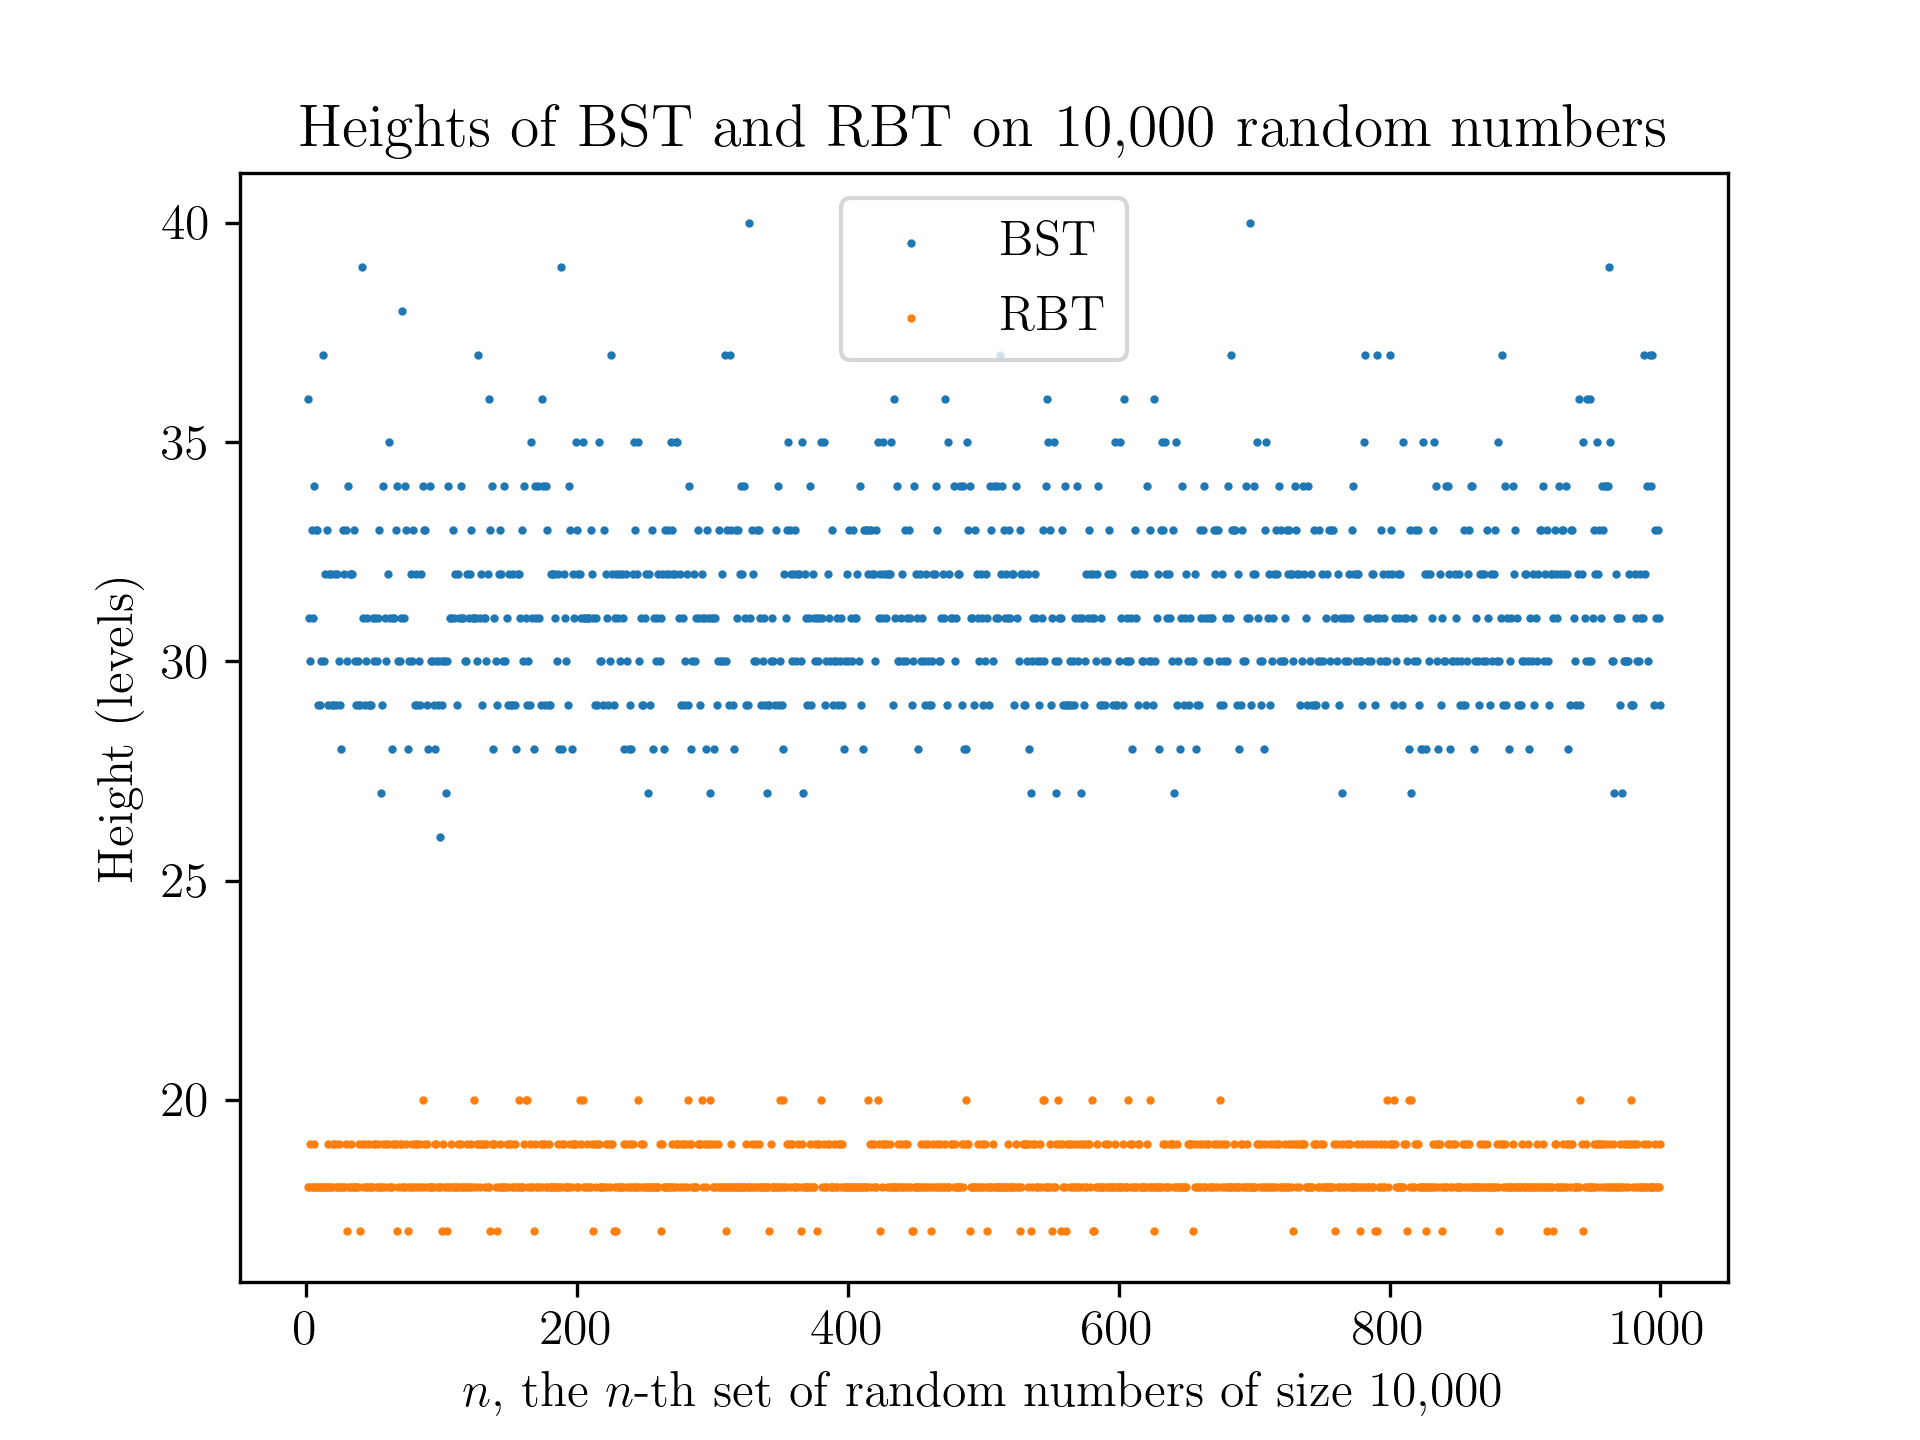
\includegraphics[width=0.8\linewidth]{rand} 
  \caption{Average heights of LLRB compared to BST on 10,000 random numbers}
  \label{fig:rand}
\end{figure}

Figure \ref{fig:near} suggests a comparison of the heights between a BST and a
RBT/LLRB tree after 10,000 insertions. More samples were taken to get a detailed
depiction of the behaviour of BST insertions in the first quarter of the sorted
factor scale. The plotted height for each sample point on the scale is an
average of 5 rounds of insertions. A significant difference of performances
between the two was observed, especially when the inversion factor is low. It is
concluded that LLBR trees have a much better worst case performance than BST.
For the remaining portion on the sorted factor scale, LLBR continued to out
perform BST in terms of tree heights. This again confirm our belief in RBT being
a strictly better searching data structure than BST.
\begin{figure}[h]
  \centering
  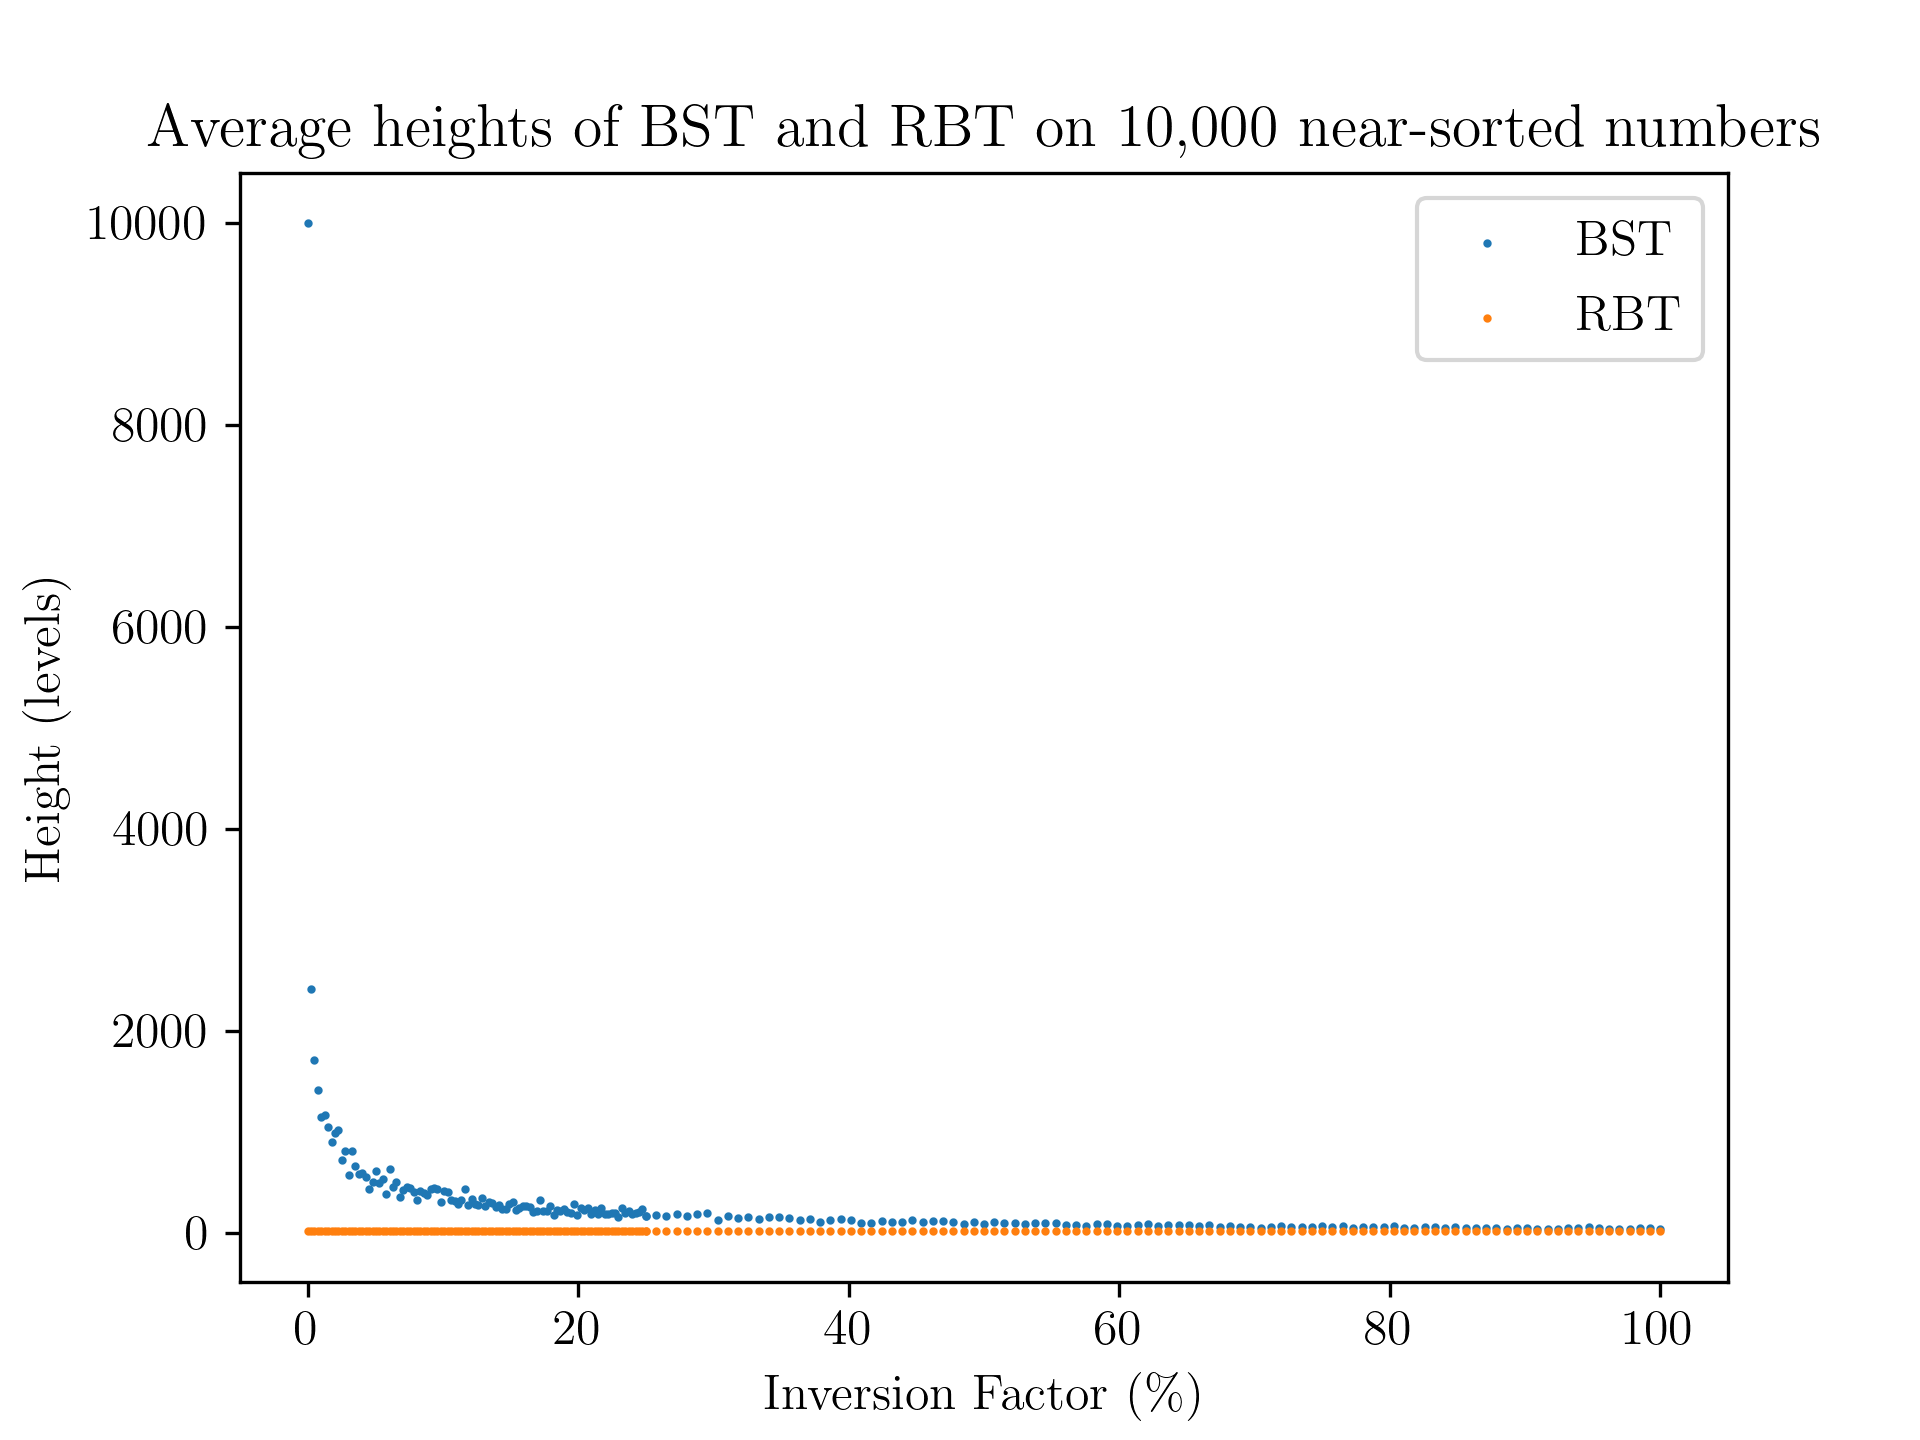
\includegraphics[width=0.8\linewidth]{near} 
  \caption{Average heights of LLBR and BST on 10,000 numbers of various sorted factor}
  \label{fig:near}
\end{figure}


\end{document}
